\documentclass{article}
\usepackage{graphicx}

\title{Axiomatic Math}
\author{William Gvozdjak}

\begin{document}

\maketitle
\begin{center}
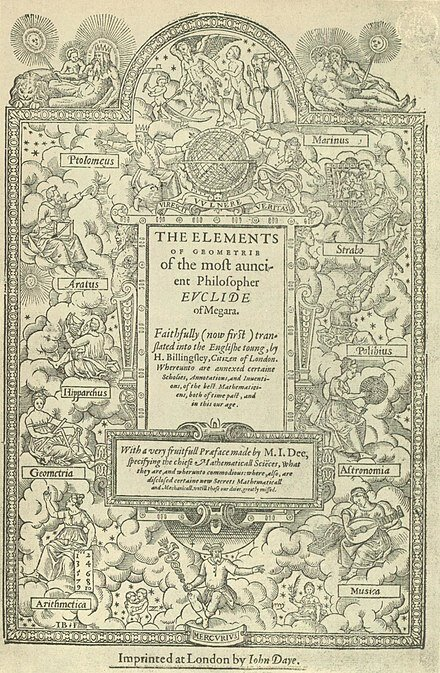
\includegraphics[scale=0.25]{Magazines/img/Vol4/euclid_elements.jpg}
\end{center}
You may have heard of the word \textit{axiom} before in the context of math. Whether through the axioms for geometry that Euclid came up with or the article \textit{Axiom of Choice} in \textit{The Circle Volume 1}, axioms are a crucial component of mathematics. But the most crucial question often eludes us until we reach college classes: what even are axioms?

To demonstrate this, we'll start with an example: linear algebra. Key to the field of linear algebra is a \textbf{vector}: a line segment starting at one point and ending at another. What defines a vector is its magnitude (its length) and its direction. Two vectors are considered equal if and only if they have equal magnitude and direction. For example, the following two vectors are equal:

\begin{center}
    \begin{asy}
        unitsize(1cm);
        draw((0, 0)--(1, 0.5), EndArrow);
        draw((1.25, 0)--(2.25, 0.5), EndArrow);
    \end{asy}
\end{center}

but these two are not:
\begin{center}
    \begin{asy}
        unitsize(1cm);
        draw((0, 0)--(1, 0.5), EndArrow);
        draw((1.75, 0)--(1.25, 0.75), EndArrow);
    \end{asy}
\end{center}

Let's suppose that the set of all 2-dimensional vectors is called $\mathbf{V}$. Then, we define the following concepts:

\begin{enumerate}
    \item \textbf{Vector addition}. If $\mathbf{v}$ and $\mathbf{w}$ are two vectors in $\mathbf{V}$, then we define $\mathbf{v}+\mathbf{w}$ as follows: place $\mathbf{w}$ so that its tail as at the tip of $\mathbf{v}$. Then $\mathbf{v}+\mathbf{w}$ is the vector with tail at the tail of $\mathbf{v}$, and tip at the tip of $\mathbf{w}$.

    \begin{center}
        \begin{asy}
            unitsize(1cm);
            draw((0, 0)--(1, 0.5), EndArrow);
            draw((1, 0.5)--(1.25, 1), EndArrow);
            draw((0, 0)--(1.25, 1), red, EndArrow);
            label("$\mathbf{v}$", (0, 0)--(1, 0.5), dir(300));
            label("$\mathbf{w}$", (1, 0.5)--(1.25, 1), dir(-30));
            label("$\mathbf{v}+\mathbf{w}$", (0, 0)--(1.25, 1), dir(130));
        \end{asy}
    \end{center}

    \item \textbf{Scalar multiplication}. If $\mathbf{v}$ is a vector in $\mathbf{V}$ and $a$ is a real number, then $a\mathbf{v}$ is the vector with magnitude $a$ times the magnitude of $\mathbf{v}$ and the same direction as $\mathbf{v}$.

    \begin{center}
        \begin{asy}
            unitsize(1cm);
            draw((0, 0)--(1, 0.5), EndArrow);
            draw((1.25, 0)--(3.25, 1), EndArrow);

            label("$\mathbf{v}$", (0, 0)--(1, 0.5), dir(130));
            label("$2\mathbf{v}$", (1.25, 0)--(3.25, 1), dir(130));
        \end{asy}
    \end{center}

    \item \textbf{Zero vector}. We define the zero vector $\mathbf{0}$ of $\mathbf{V}$ to be a vector with magnitude $0$.
\end{enumerate}

Now, we observe the following properties, where $\mathbf{u}$, $\mathbf{v}$, and $\mathbf{w}$ are two vectors in $\mathbf{V}$.

\begin{enumerate}
    \item $a\mathbf{v}\in\mathbf{V}$, $\mathbf{v}+\mathbf{w}\in\mathbf{V}$. Formally, we say that $\mathbf{V}$ is \textbf{closed} under vector addition and scalar multiplication. This is obvious: the operations we defined above result in elements of $\mathbf{V}$.
    \item $\mathbf{v}+\mathbf{w}=\mathbf{w}+\mathbf{v}$ (vectors in $\mathbf{V}$ are \textbf{commutative}). Verify this using the definition of vector addition above!
    \item $(\mathbf{u}+\mathbf{v})+\mathbf{w}=\mathbf{u}+(\mathbf{v}+\mathbf{w})$ (vectors in $\mathbf{V}$ are \textbf{associative}).
    \item $\mathbf{v}+\mathbf{0}=\mathbf{v}$ ($\mathbf{0}$ is the \textbf{additive identity} of $\mathbf{V}$).
    \item $0\mathbf{v}=\mathbf{0}$.
    \item $1\mathbf{v}=\mathbf{v}$ ($1$ is the \textbf{multiplicative identity}).
    \item $a(b\mathbf{v})=(ab)\mathbf{v}$.
    \item $a(\mathbf{v}+\mathbf{w})=a\mathbf{v}+a\mathbf{w}$ (scalar multiplication is \textbf{distributive} over vector addition).
    \item $(a+b)\mathbf{v}=a\mathbf{v}+b\mathbf{v}$.
\end{enumerate}

Now, we introduce the crucial step: \textbf{abstracting away} from these types of vectors. In other words, instead of \textit{observing} the above 9 properties from vectors, we will \textit{assume} that the properties are true, and look at what potential objects satisfy these properties. Each ``type'' of object that does satisfy these properties forms a \textbf{vector space}.

Formally, a vector space $\mathbf{V}$ is a set of objects known as \textit{vectors} (notice that these vectors may or may not be the same vectors as before! The entire point of defining a vector space is to create a sort of template for a generic set of objects). For these objects, two types of operations must be defined: scalar multiplication $a\mathbf{v}$ and vector addition $\mathbf{v}+\mathbf{w}$. The zero vector $\mathbf{0}$ must exist. Then, for all vectors $\mathbf{u}$, $\mathbf{v}$, and $\mathbf{w}$ in $\mathbf{V}$ and all real numbers $a$ and $b$, the following properties must be true:

\begin{enumerate}
    \item $a\mathbf{v}\in\mathbf{V}$, $\mathbf{v}+\mathbf{w}\in\mathbf{V}$

    \item $\mathbf{v}+\mathbf{w}=\mathbf{w}+\mathbf{v}$

    \item $(\mathbf{u}+\mathbf{v})+\mathbf{w}=\mathbf{u}+(\mathbf{v}+\mathbf{w})$

    \item $\mathbf{v}+\mathbf{0}=\mathbf{v}$

    \item $0\mathbf{v}=\mathbf{0}$.

    \item $1\mathbf{v}=\mathbf{v}$

    \item $a(b\mathbf{v})=(ab)\mathbf{v}$.

    \item $a(\mathbf{v}+\mathbf{w})=a\mathbf{v}+a\mathbf{w}$

    \item $(a+b)\mathbf{v}=a\mathbf{v}+b\mathbf{v}$.
\end{enumerate}

These 9 properties are known as \textbf{axioms} (in this special case, they're known as the \textbf{axioms of vector spaces}): they are certain requirements that must be met in order for something to be called a vector space. Notice that the set of two-dimensional vectors that we discussed earlier forms a vector space, as they satisfy all of the above axioms. There exist many other vector spaces as well: function spaces, polynomial spaces, and much more.

So, why do we care? The answer is: using these measly 9 axioms, it turns out that we can prove many interesting properties about vector spaces. Just by satisfying these axioms, we can infer fascinating ideas about a set of objects, which we can use to explore and better understand them.

Axioms are not just used in linear algebra: they're used almost everywhere, from group theory to geometry. So be sure to take a moment and appreciate the significance of axioms in the field you're exploring the next time you encounter a mathematical topic.

\begin{center}
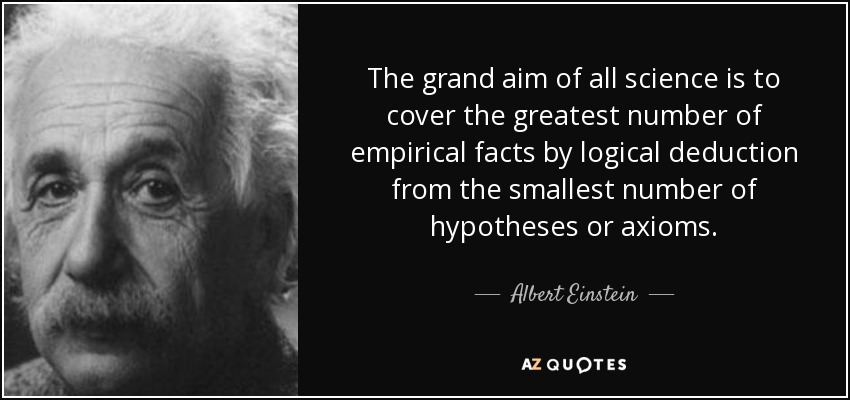
\includegraphics[scale=0.18]{Magazines/img/Vol4/albert_einstein_quote.jpg}
\end{center}
\end{document}